% úvod
%Konečně se dostáváme k něčemu reálnému. Zde popíši hardwarovou část řešení tj. Co vlastně bude měřit, čím budu 
%měřit\ldots

% měřící stanice
\section{Měřící stanice}
\begin{figure}[H]
    \centering
    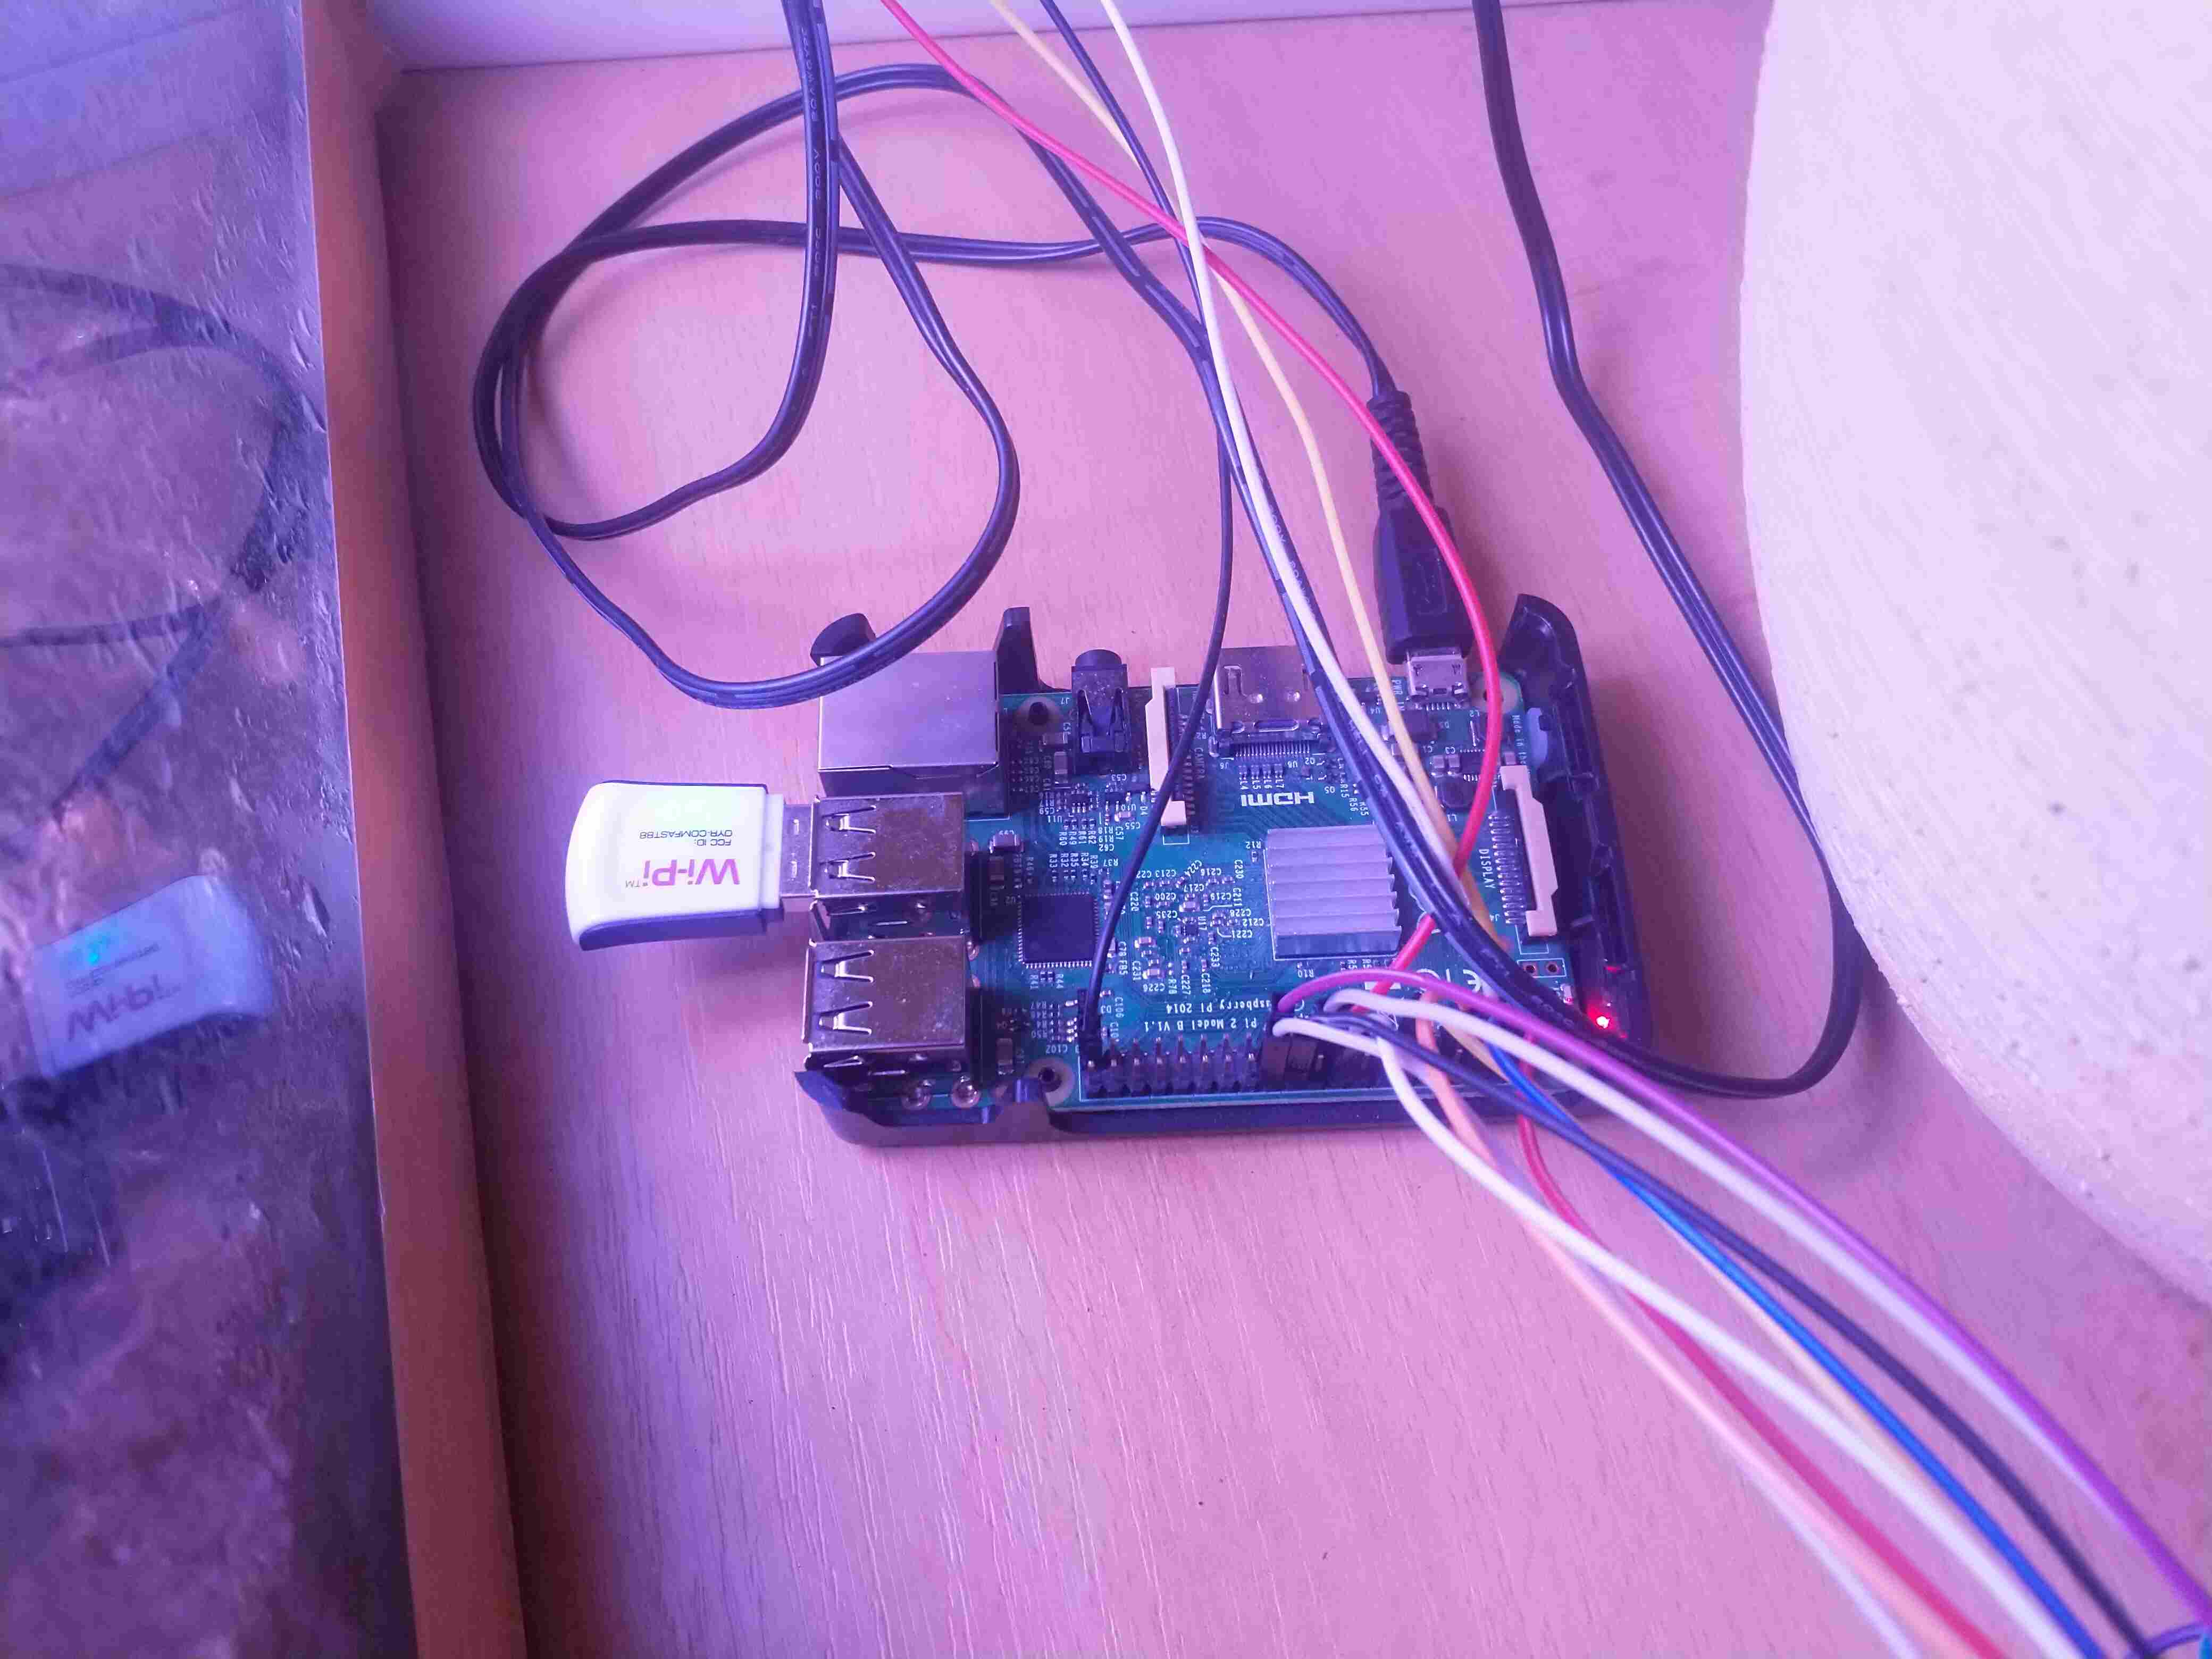
\includegraphics[width=0.8\textwidth]{RPi2.jpg}
    \caption{Raspberry pi 2}
\end{figure}
Možných základů pro měřící stanici, jednodeskových počítačů, je dnes na trhu mnoho od různých osmibitů, až po počítače 
na architektuře ARM,  které dosahují výkonu srovnatelného s mobilními telefony. Já jsem pro mé řešení zvolil Raspberry 
Pi ve verzi 2 a to z několika důvodů. Jednak ho mám k dispozici a dále mi nabízí běžící Linux a tudíž za mne řeší 
spoustu problémů, od síťové komunikace, po třeba synchronizaci času. Navíc mám k dispozici spoustu digitálních pinů pro 
připojení různých senzorů, též mám vyřešené i místní úložiště, data se mohou ukládat na SD kartu ze které běží celý 
systém a výrazně to zjednodušuje vývoj, poněvadž mohu nahrávat nové verze programů vzdáleně, a i vzdáleně sledovat 
jejich běh, což je pro mě výhodné, neb terárium nemám v pokoji, kde programuji. Samozřejmě že toto řešení má i své 
nevýhody. Například v případě, že bych chtěl měřit analogové hodnoty, bych musel dokupovat převodník z analogového 
signálu na digitální, či v případě nutnosti rozšíření na více míst, by to nebylo ekonomicky výhodné, přeci jen Raspberry 
Pi stojí kolem 1000 Kč. Nebo pokud bych chtěl zařízení napájet z akumulátoru, tak s odběrem kolem půl ampéru by moc 
dlouho nevydržel. Avšak v případě zmíněných problémů mi zvolené celkové řešení umožňuje poměrně komfortně změnit základ 
stanice na něco vhodnějšího, za předpokladu, že se zvolená deska zvládne připojit na lokální síť. Například mohu použít 
oblíbenou desku ESP8266 či ESP32, které se cenově pohybují v řádu stokorun, pinů mají dostatek, disponují Wifi čipem 
a umožňují použití nízko odběrových módů při běhu na baterii.

% senzory
\section{Senzory}
% BME280
\subsection{BME280}
Pro měření hodnot v teráriu jsem zvolil senzor BME280 teploty vlhkosti a tlaku vzduchu od firmy Bosh s cenovkou kolem 
100 Kč. Navíc díky sběrnici \gls{I2C} mi z terária vedou pouze čtyři dráty.

\begin{figure}[H]
		\centering
    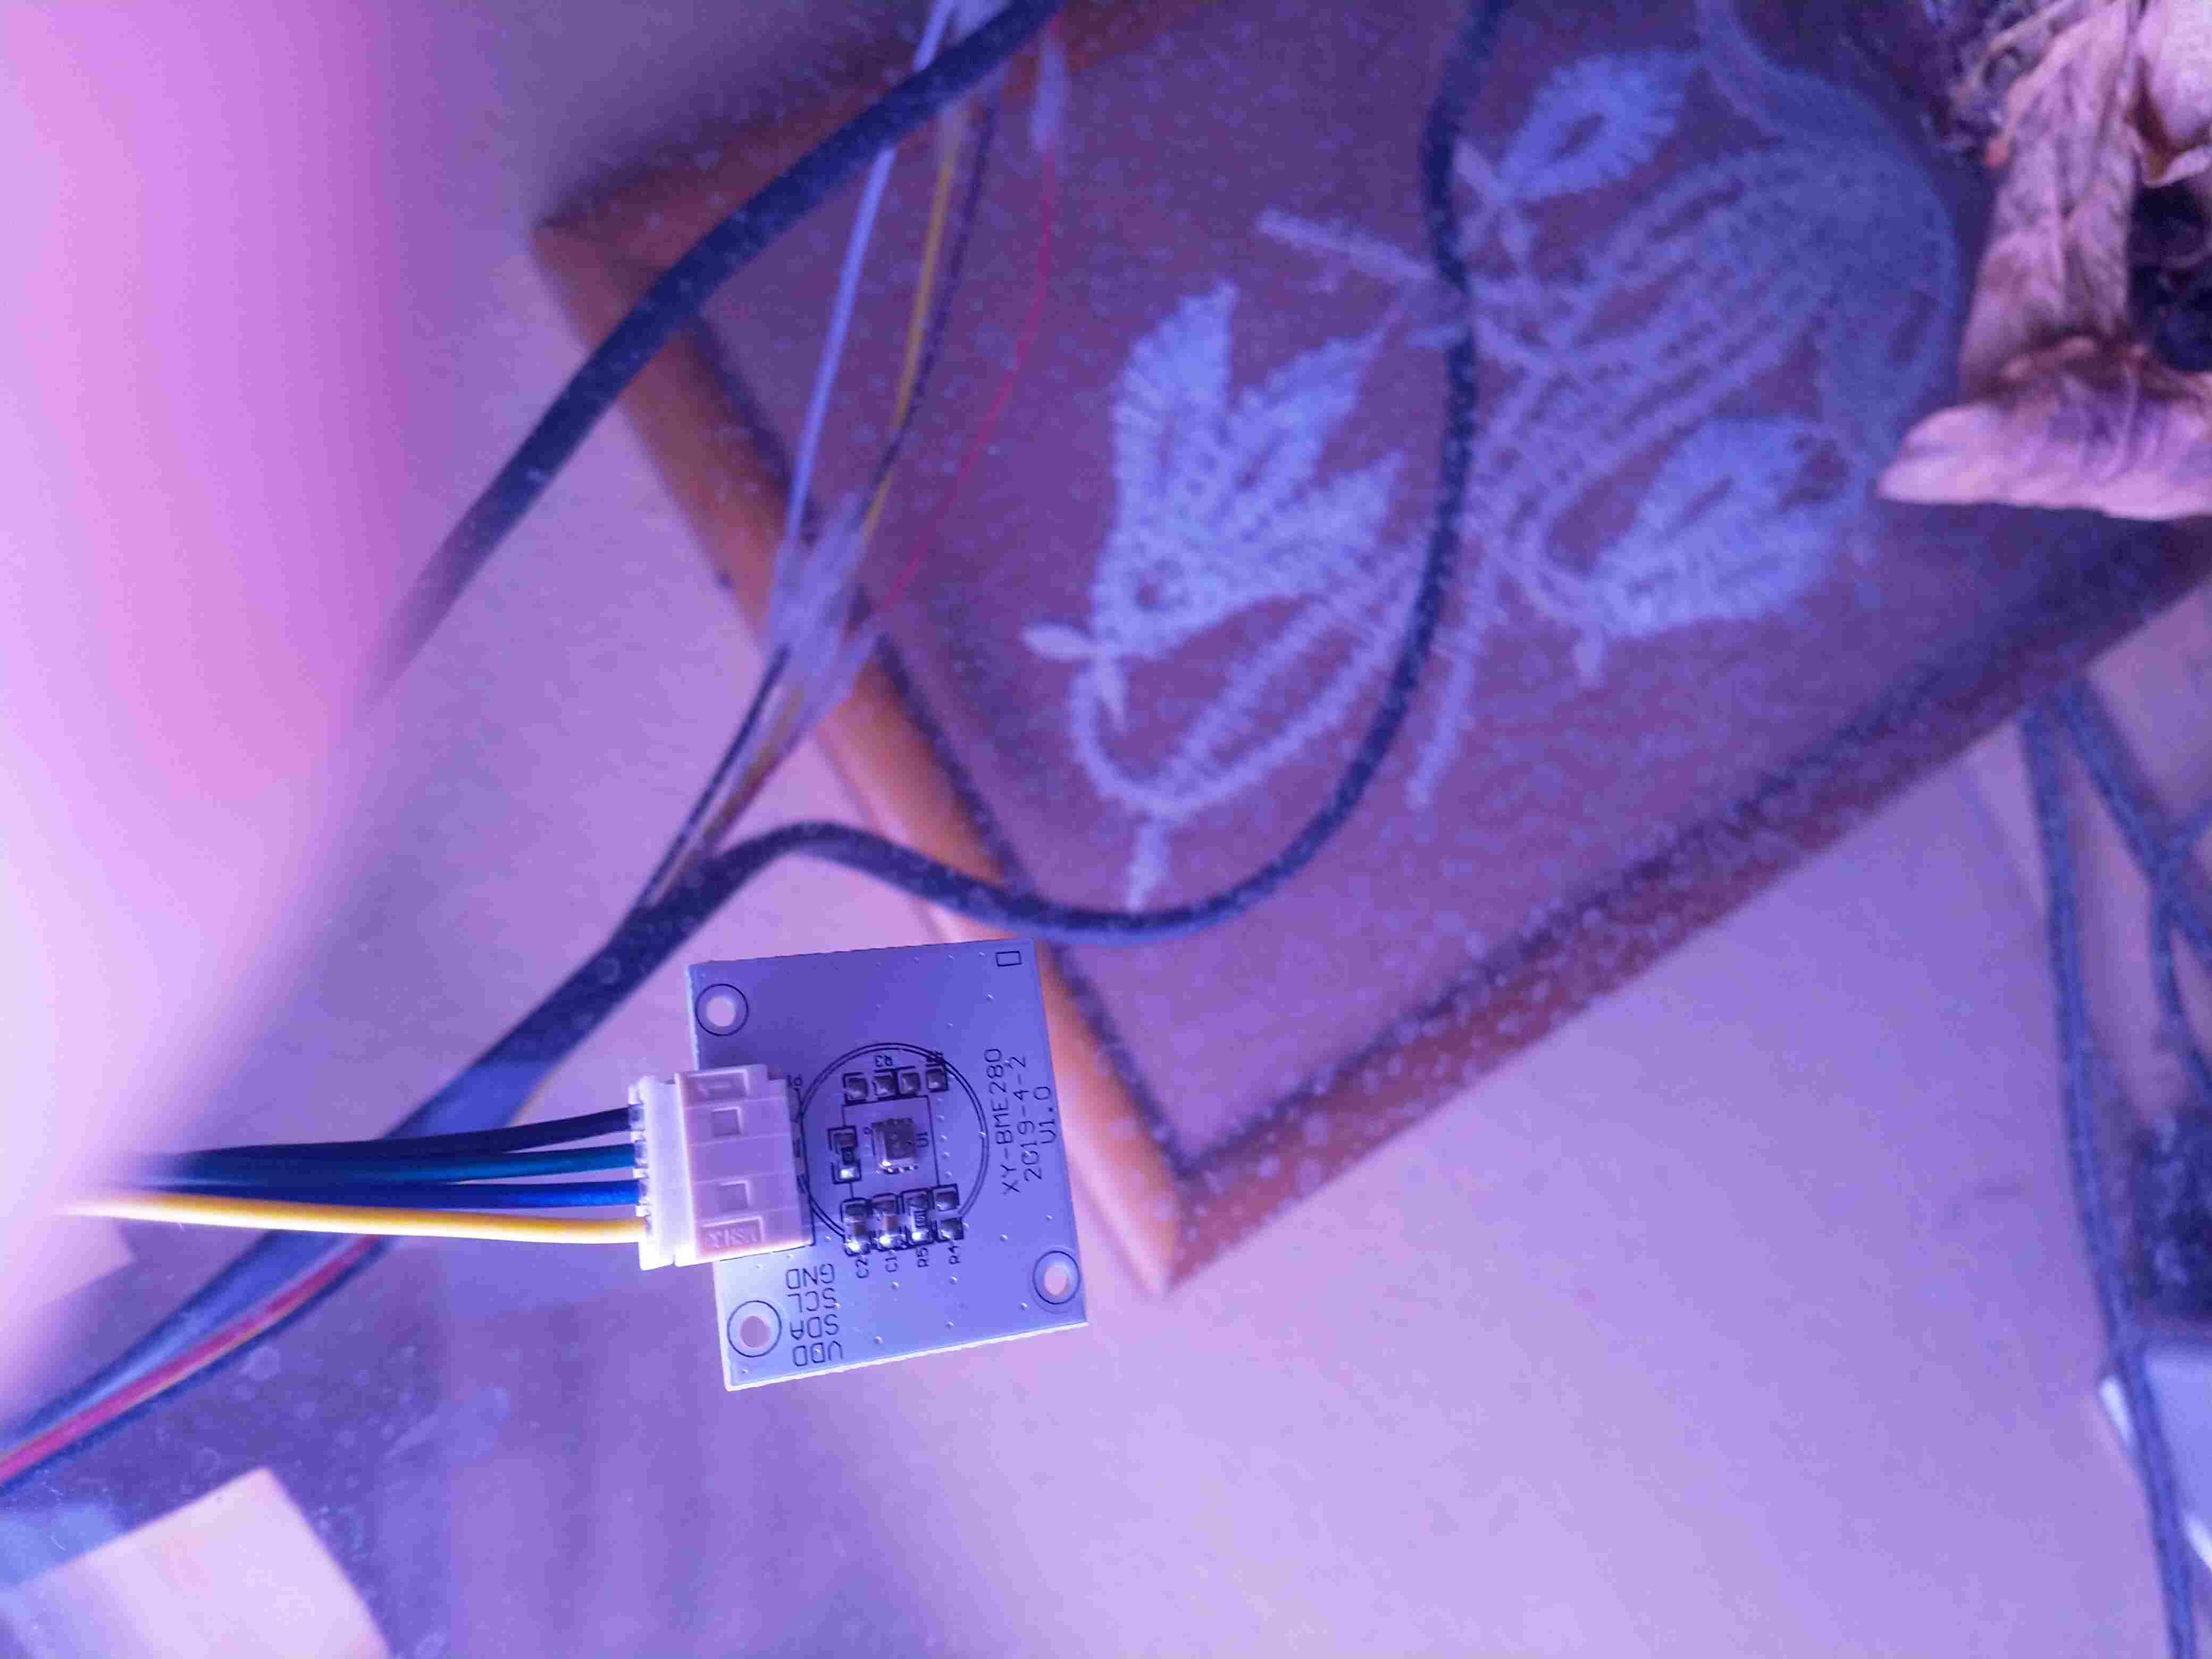
\includegraphics[angle=270,width=0.5\textwidth]{BME280.jpg}
    \caption{Modul s BME280, stříbrný čtvereček uprostřed}
\end{figure}

\begin{table}[H]
    \centering
    \begin{tabular}{|l|c|}
        \hline
        \multicolumn{2}{|c|}{Teplota} \\ \hline
        \hline
        Rozsah & -40 až +85\textdegree C \\ \hline
        Rozlišení & 0,01\textdegree C \\ \hline
        Přesnost & $\pm$ 1\textdegree C \\ \hline
        \hline
        \multicolumn{2}{|c|}{Vlhkost} \\ \hline
        \hline
        Rozsah & 0 až 100\% \\ \hline
        Rozlišení & 0,008\% \\ \hline
        Přesnost & $\pm$2\% \\ \hline
        \hline
        \multicolumn{2}{|c|}{Tlak} \\ \hline
        \hline
        Rozsah & 300 až 1100 hPa \\ \hline
        Rozlišení & 0,18 Pa \\ \hline
        Přesnost & 1 $\pm$ Pa \\ \hline
    \end{tabular}
    \caption{Parametry BME280}
\end{table}

% DS18B20
\subsection{DS18B20}
Za účelem případné další analýzy, jsem umístil pár senzorů i mimo terárium, abych mohl sledovat závislost teploty vně 
a uvnitř.Jako hlavní senzor teploty jsem použil DS18B20 vyvinutý firmou Dallas s cenou čínské kopie asi 35 Kč. Jde o můj 
oblíbený senzor, poněvadž je přesný, snadno použitelný a díky sběrnici \gls{onewire} mu stačí pouze tři, případě dva 
dráty.

\begin{figure}[H]
    \centering
    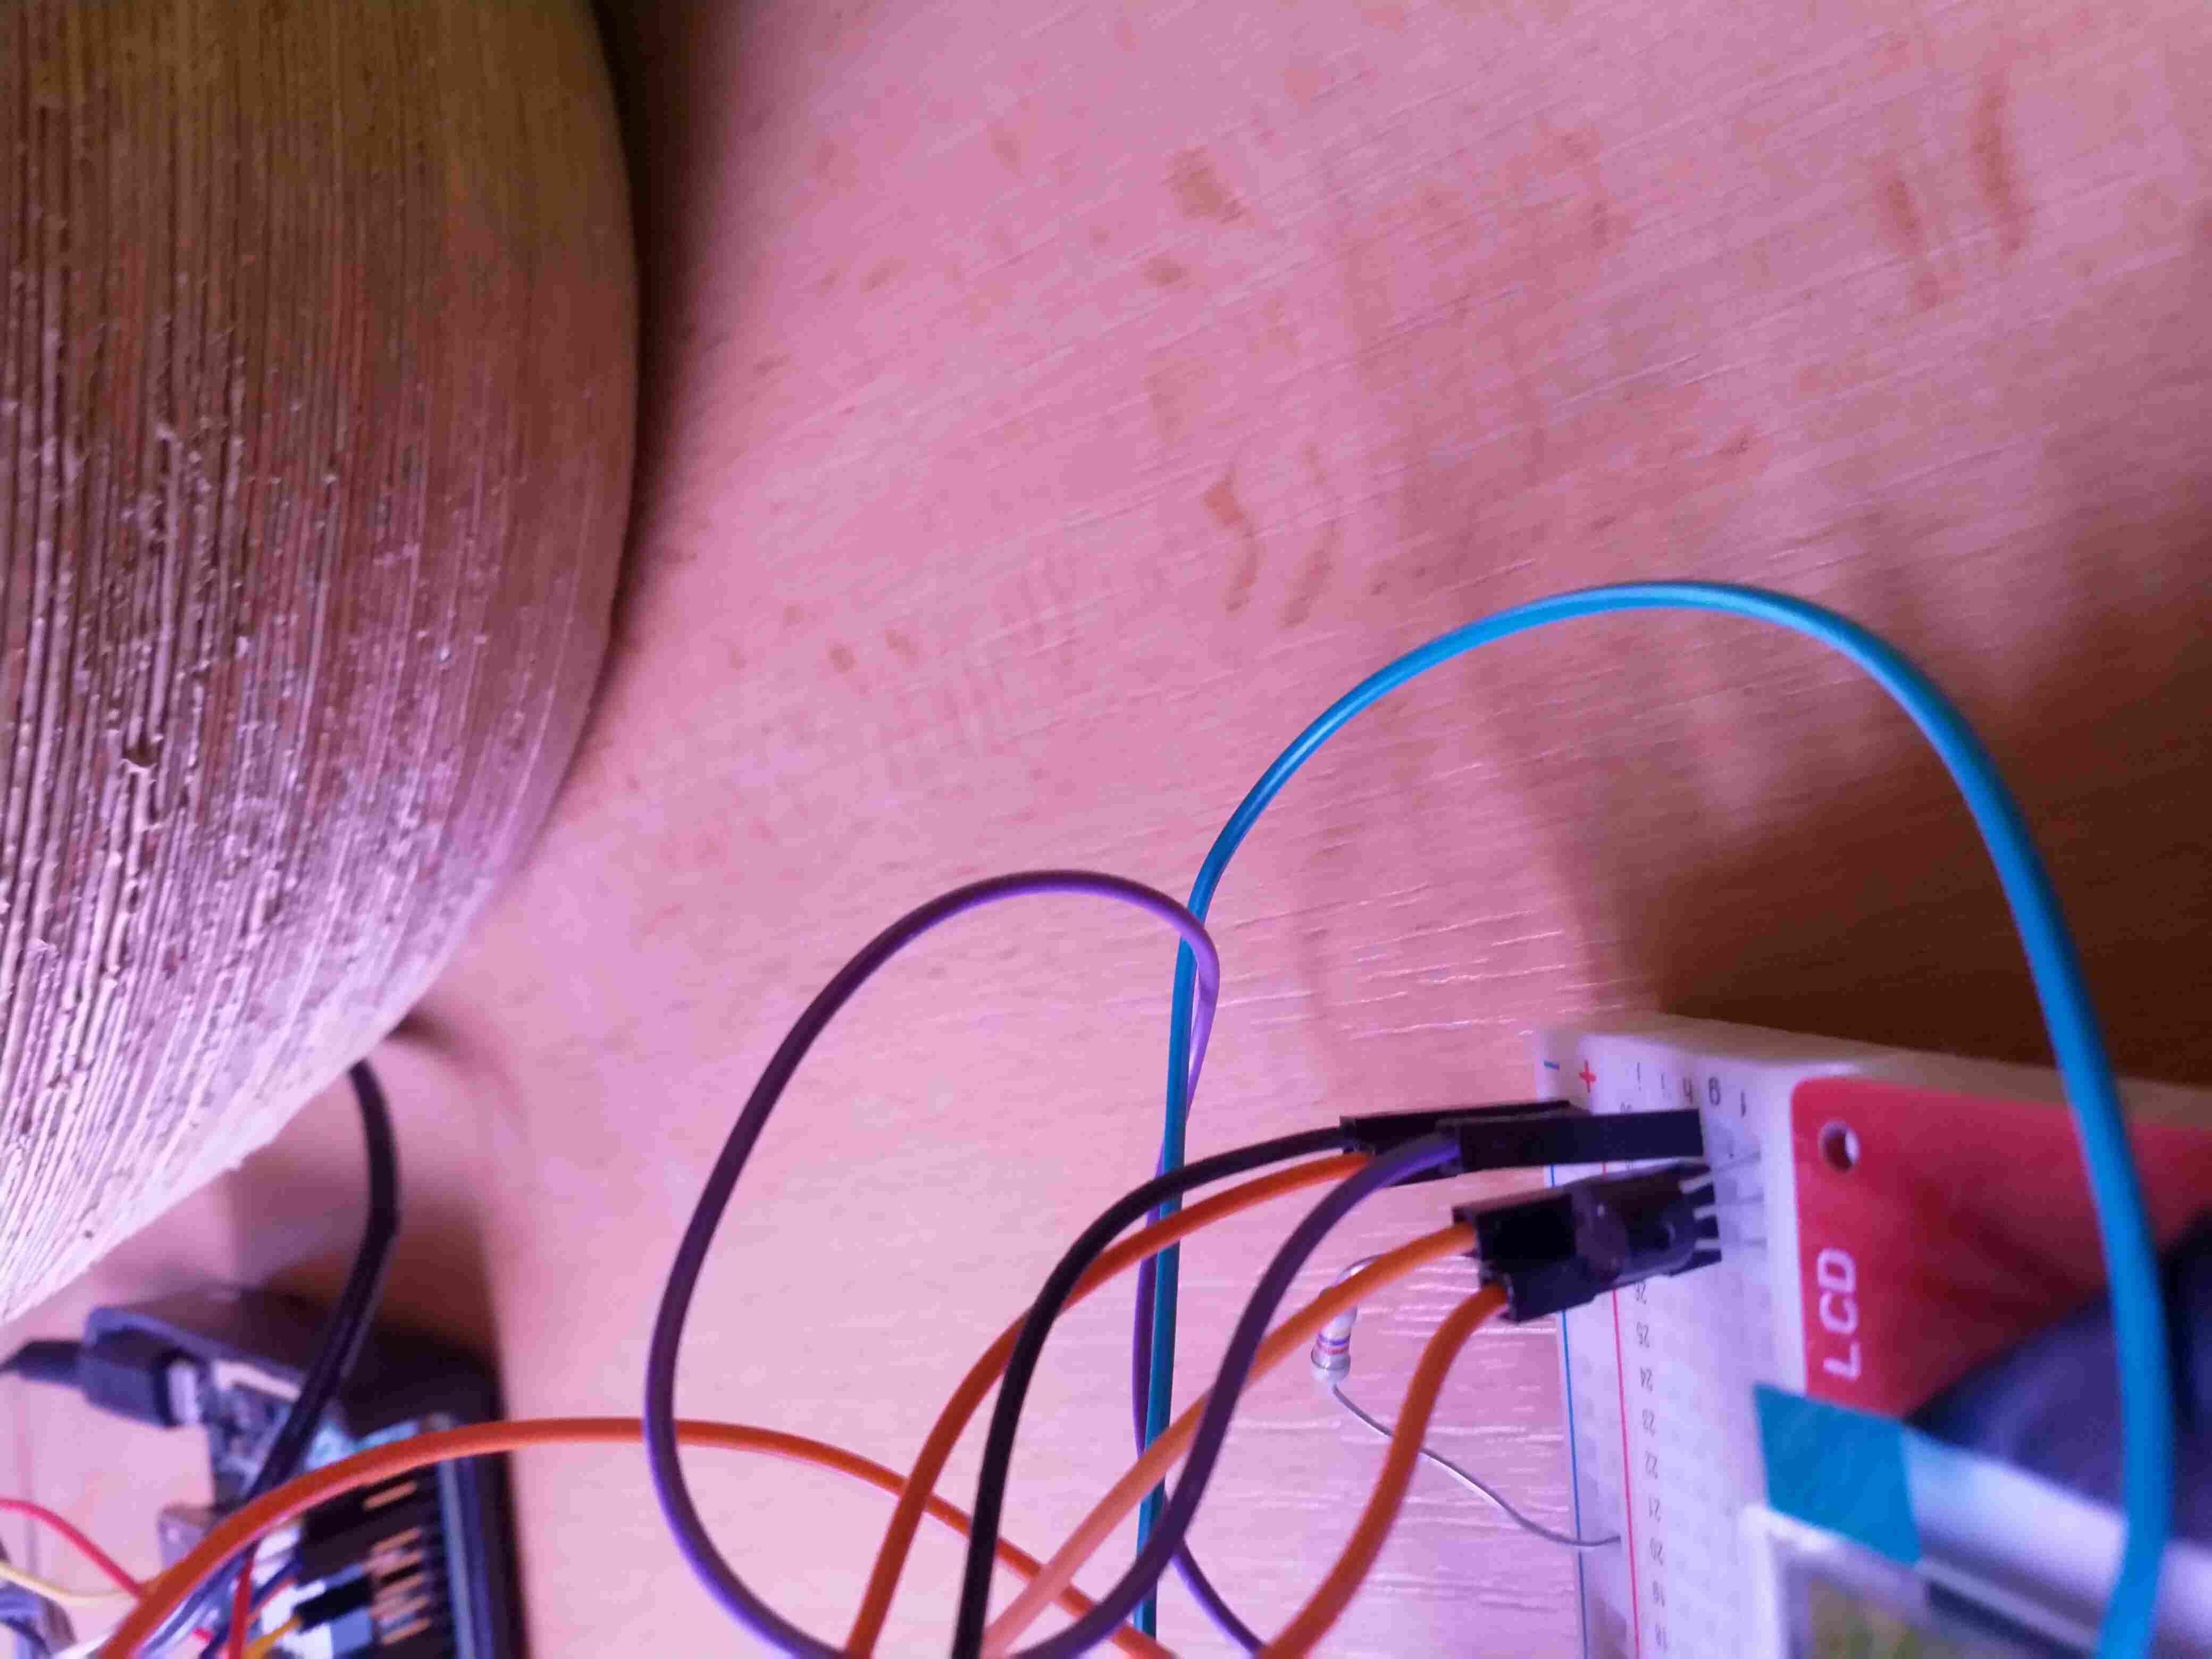
\includegraphics[angle=270,width=0.5\textwidth]{DS18B20.jpg}
    \caption{DS18B20, pouzdro TO-92}
\end{figure}

\begin{table}[H]
    \centering
    \begin{tabular}{|l|c|}
        \hline
        \multicolumn{2}{|c|}{Teplota} \\ \hline
        \hline
        Rozsah & -55 až +125\textdegree C \\ \hline
        Rozlišení & 0,0625\textdegree C \\ \hline
        Přesnost & $\pm$ 0,5\textdegree C \\ \hline
    \end{tabular}
    \caption{Parametry DS18B20}
\end{table}

% DHT11
\subsection{DHT11}
Pro měření vlhkosti vně terária jsem použil oblíbený senzor teploty a vlhkosti DHT11 s cenovkou kolem 40 Kč. Senzor 
teploty jsem zdvojil z důvodu velké nepřesnosti tohoto modelu. S tímto senzorem jsem měl největší problémy, zejména díky 
jeho nestandardní sběrnici, která připomíná \gls{onewire}, ale používá jiný komunikační protokol.

\begin{figure}[hbt]
    \centering
    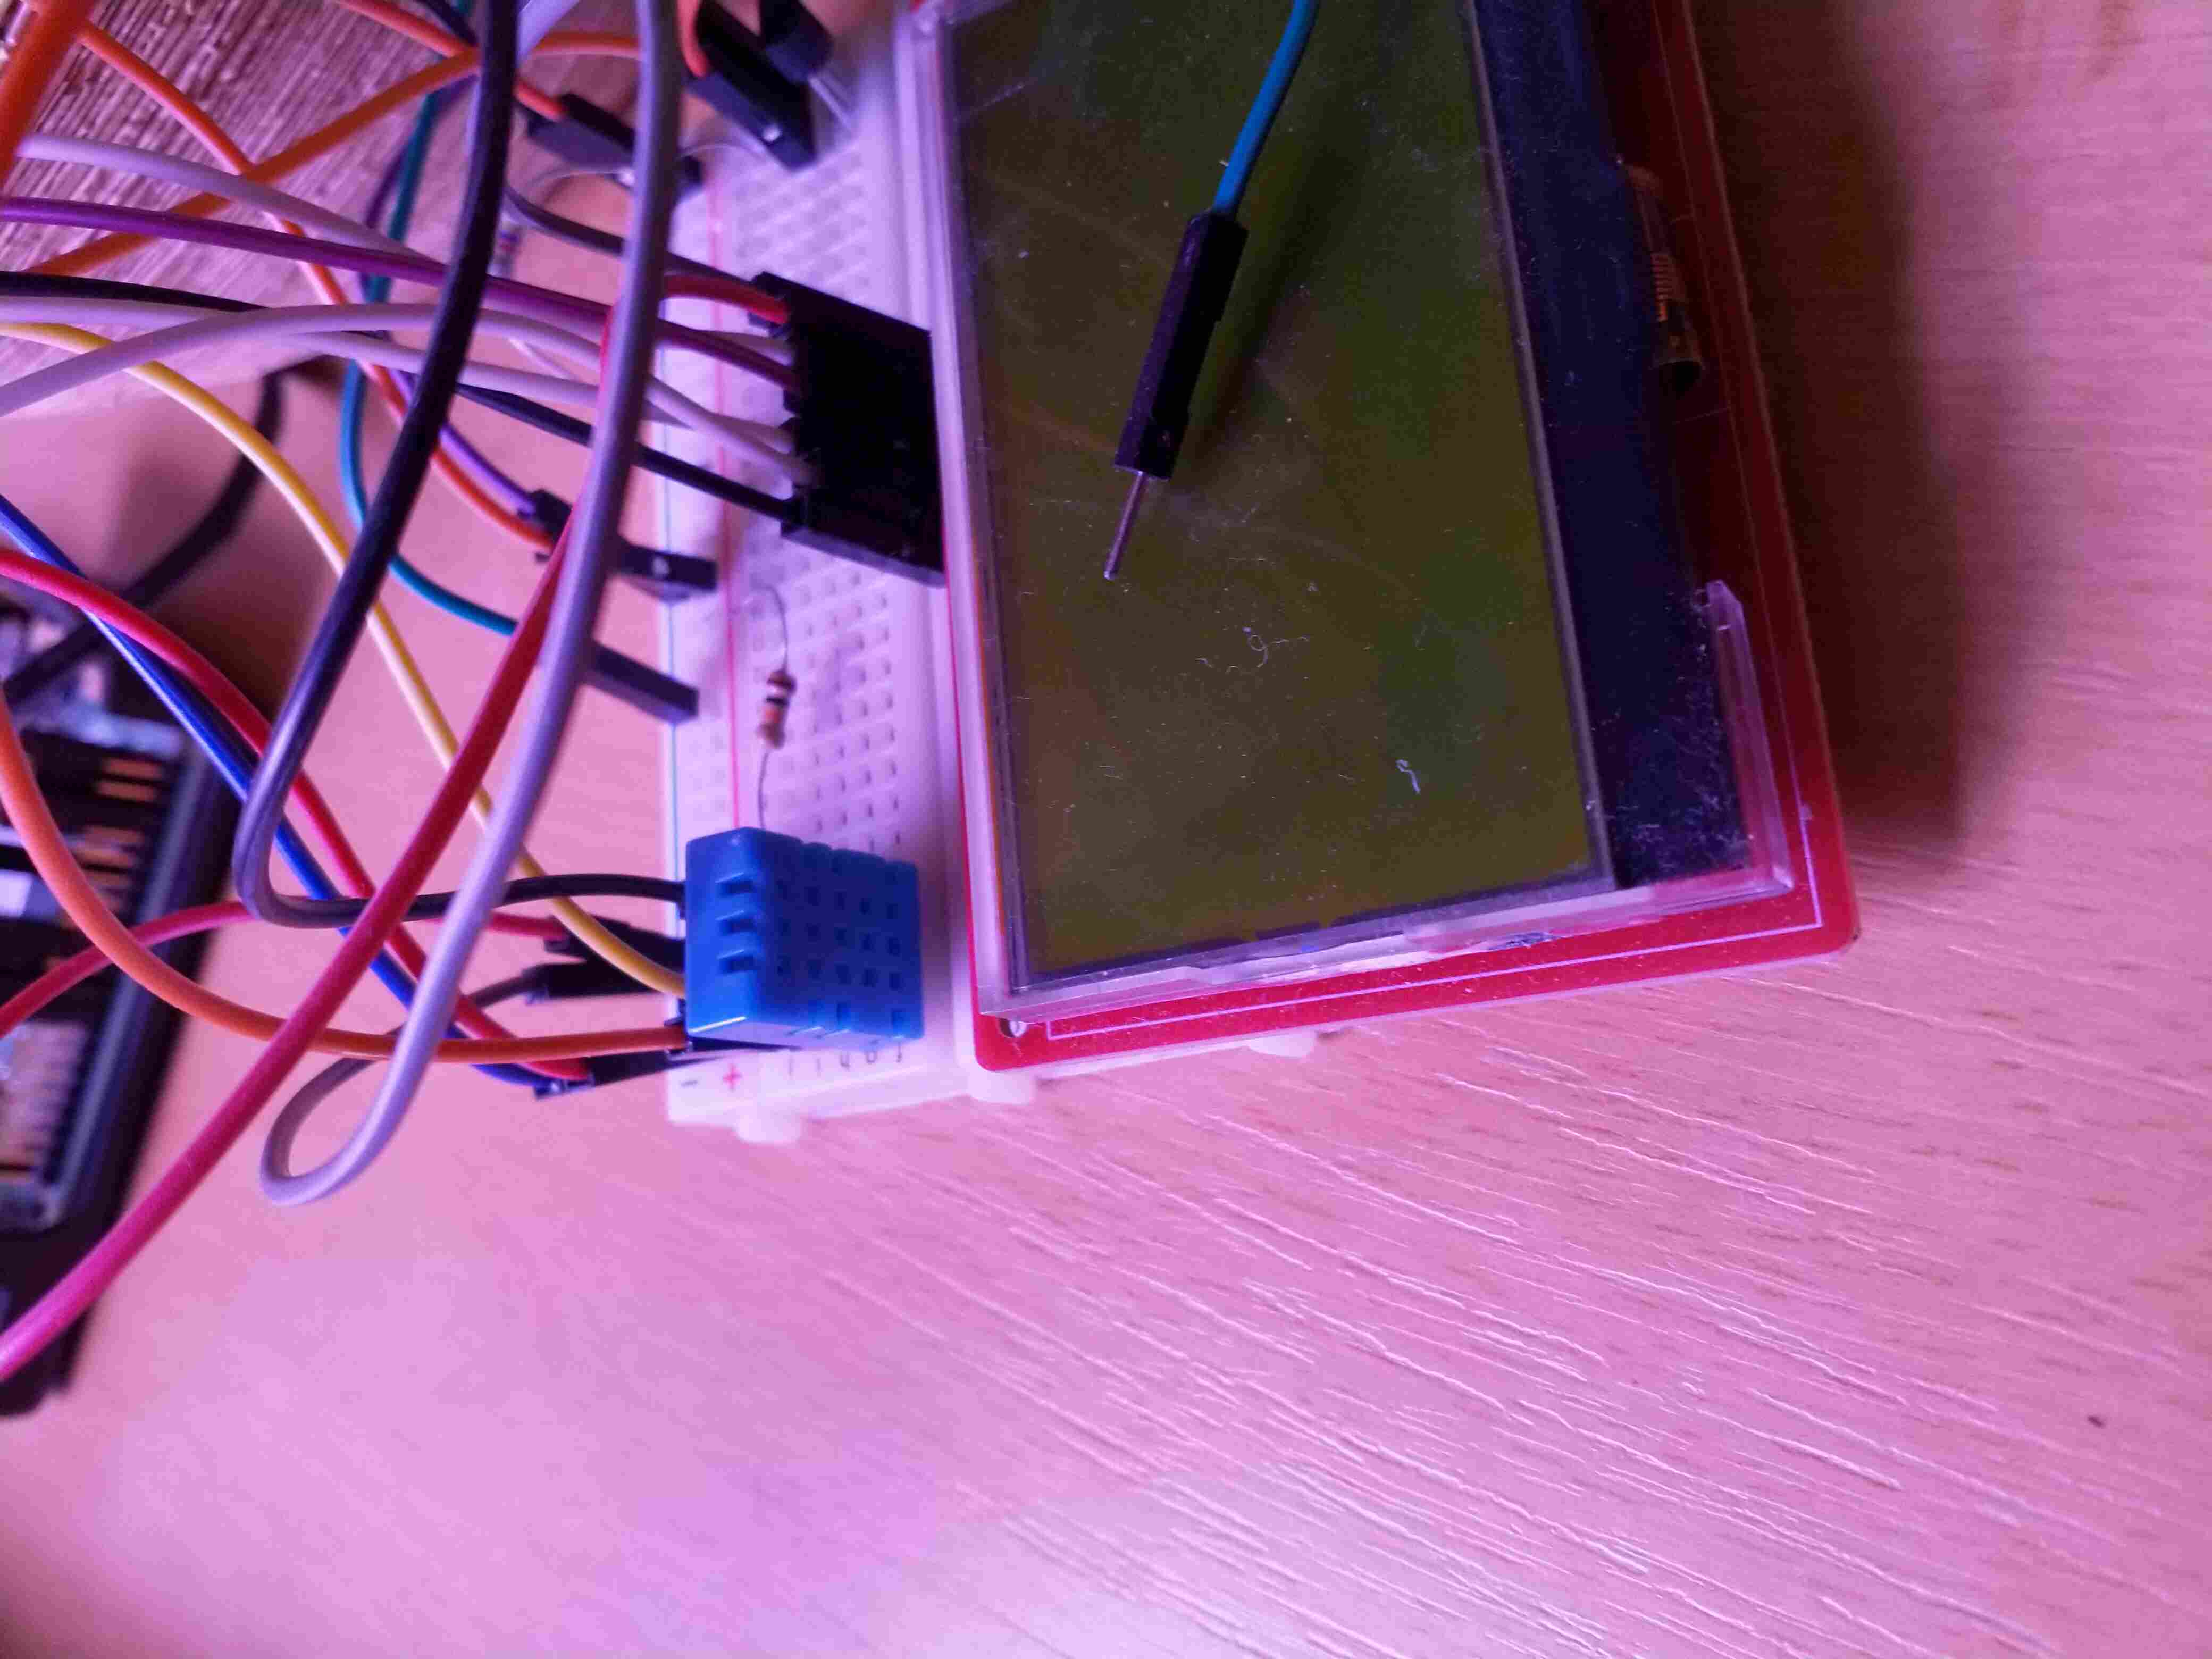
\includegraphics[angle=270,width=0.5\textwidth]{DHT11.jpg}
    \caption{DHT11, modrý obdélníček}
\end{figure}

\begin{table}[H]
    \centering
    \begin{tabular}{|l|c|}
        \hline
        \multicolumn{2}{|c|}{Teplota} \\ \hline
        \hline
        Rozsah & 0 až +50\textdegree C \\ \hline
        Rozlišení & 1\textdegree C \\ \hline
        Přesnost & $\pm$ 2\textdegree C \\ \hline
        \hline
        \multicolumn{2}{|c|}{Vlhkost} \\ \hline
        \hline
        Rozsah & 20 až 90\% \\ \hline
        Rozlišení & 1\% \\ \hline
        Přesnost & $\pm$5\% \\ \hline
    \end{tabular}
    \caption{Parametry DHT11}
\end{table}

% gateway
\section{Brána}
Jako brána pro komunikaci s internetem se dá taky použit téměř cokoli, ale přeci jen jsou na ní kladeny větší nároky než 
na měřící stanici. Mimo nutnosti možnosti připojení do sítě je též třeba výpočetní výkon a paměť, dostatečná na 
komunikaci s cloudem, řešení šifrování, běh nějakého message brokera\ldots, tedy nejlépe nějakou desku s operačním 
systémem, který mi tohle všechno umožní. Já jsem zvolil opět Raspberry Pi, tentokrát ve verzi 3 opět z velmi 
jednoduchého důvodu, už mi doma běží, jako takový domácí server.
